\chapter{Ryzyko kredytowe}

\section{Rola oceny ryzyka kredytowego we spółczesnych gospodarkach rynkowych}

\subsection{Wprowadzenie}

Wraz z postępem globalizacji, międzynarodowe rynki finansowe utworzyły strukturę przypominającą sieć naczyń połączonych. Zdarzenia występujące nawet w obrębie gospodarek pojedynczych państw mogą mieć znamienny wpływ na ogólnoświatową kondycję ekonomiczną. Biorąc pod uwagę, że stan współczesnych rynków ekonomicznych jest silnie skorelowany z kondycją instytucji finansowych takich jak banki, których główna działalność opiera się na kredytowaniu podmiotów zarówno prywatnych i instytucjonalnych, można jednoznacznie stwierdzić, że prawidłowa i precyzyjna ocena ryzyka kredytowego jest rzeczą absolutnie niezbędną z punktu widzenia zachowania równowagi na rynkach finansowych.

Przykładem katastrofalnych skutków, jakie niesie za sobą błąd w modelowaniu tego typu ryzyka jest wielki kryzys finansowy przypadający na lata 2007 – 2015, który zostanie dokładniej opisany w dalszej części artykułu. Ze względu na istotność i wagę tego problemu istnieje szereg dyrektyw międzynarodowych nakładających stosowne regulacje na instytucje finansowe, aby stosowane przez nie praktyki w sferze kredytowania nie mogły doprowadzić do poważnych zachwiań w gospodarkach światowych na miarę wspomnianego kryzysu.

Najbardziej istotnymi dokumentami tego typu są normy Basel II i Basel III wprowadzone przez Basel Comittee on Banking Supervision (BCBS) – organ powołany przez banki centralne sprawujący szeroko pojęty nadzór nad praktykami całego sektora bankowego.

\subsection{Definicja ryzyka kredytowego}

Ryzykiem kredytowym nazywamy ryzyko zaistnienia takich okoliczności, z powodu których wartość portfela kredytów i papierów wartościowych instytucji ulegnie wahaniom (spadkowi) z powodu nagłych i nieprzewidzianych zmian zdolności kredytowej kredytobiorców lub partnerów inwestycyjnych.

Podstawowym podziałem ryzyka kredytowego jest:
\begin{itemize}
\item Ryzyko niewypłacalności, czyli wystąpienia opóźneń bądź całkowitego zaprzestania spłaty kredytu
\item Ryzyko spadku zdolności kredytowej (Credit Ratings)
\end{itemize}

Z punktu widzenia projektowania platformy wspomagającej ocenę ryzyka kredytowego istotna jest ta druga podgrupa.

\subsection{Metody oceny ryzyka kredytowego}

Kluczową miarą z punktu widzenia zarządzania ryzykiemr kredytowym jest RWA - Risk-weighted Assets. RWA składa się z:

\begin{itemize}
\item Sumy wag ryzyka pomnożonych przez kapitał pozycji uwzględnainej w bilansie
\item Sumy wag ryzyka pomnożonych przez
ekwiwalent kredytu dla pozycji nie uwzględnianej w bilansie (np. instrumenty pochodne)
\end{itemize}

\begin{equation} \label{eq:RWA}
RWA = \sum_{i=1}^{N}\alpha_{i}E_{i} + \sum_{j=1}^{M}w_{j}C_{j}
\end{equation}
Gdzie:
\begin{itemize}
	\item $\alpha_{i}$ - waga ryzyka dla i-tej pozycji uwzględnianej w bilansie
	\item $E_{i}$ - kapitał i-tej pozycji uwzględnianej w bilansie
	\item $w_{j}$ - waga ryzyka dla j-tej pozycji nie uwzględnianej w bilansie
	\item $C_{j}$ - ekwiwalent kredytu dla j-tej pozycji nie uwzględnianej w bilansie
\end{itemize}

Formuła (\ref{eq:RWA}) jest najbardziej ogólną formą modelu służącego bankom do wyznaczenia wartości RWA. Następnie w oparciu o tę wartość wyznaczany jest wymagany kapitał zabezpieczający udzielone kredyty – stanowi on 8\% RWA. Istnieją dwa podstawowe podejścia do zagadnienia modelowania ryzyka:

\begin{itemize}
\item Podejście standaryzowane (ang. \textit{Standardized Approach})
\item Podejście oparte na wewnętrznym ratingu (ang. \textit{Internal-Rating Based Approach})
	\begin{itemize}
	\item Foundation IRB
	\item Advanced IRB
	\end{itemize}
\end{itemize}

\subsubsection{Standardized approach}

Wartości wag do wzoru (\ref{eq:RWA}) dostarcza krajowy regulator. Są one zdefiniowane dla poszczególnych klas kredytobiorców, np. korporacja, bank, instytucja rządowa. Jest to najprostsza forma wyznaczania wartości RWA stosowana jedynie przez mniejsze instytucje, które nie mogą sobie pozwolić na stosowanie bardziej zaawansowanych metod modelowania ryzyka.

\subsubsection{Internal-RatingBasedApproach}
W przypadku wariantu “Foundation” bank musi wyznaczyć jedynie prawdopodobieństwo niewypłacalności (ang. \textit{Probability of Default}), natomiast w przypadku metody zaawansowanej (Advanced IRB) oprócz PD bank musi wyznaczyć stratę przy (całkowitej) niewypłacalności (ang. \textit{Exposure at Default}) oraz faktyczną stratę (ang. Loss Given Default), która określa procentowy stosunek poniesionych strat do straty przy niewypłacalności (EAD). Otrzymane wartości pozwalają na wyznaczenie wartości RWA w oparciu wewnętrzy model banku, pod warunkiem, że jego specyfikacja została dostarczona krajowemu regulatorowi oraz pomyślnie przeszła weryfikację poprawności i zgodności z obowiązującymi normami.

\section{Kryzys na światowych rynkach finansowych po roku 2007}

\subsection{Geneza}

Genezy gólnoświatowego kryzysu gospodarczego rynków finansowych należy szukać na rynku pożyczek wysokiego ryzyka udzielanych w USA osobom o niewystarczających możliwościach finansowych (ang. subprime mortgage). Pożyczki te były wykorzystywane jako zabezpieczenie obligacji strukturyzowanych emitowanych przez instytucje finansowe – w szczególności duże banki. Z powodu hossy na rynku nieruchomości i wprowadzenia mniej restrykcyjnych przepisów prawnych, instytucje ratingowe wystawiały rzeczonym obligacjom zawyżone oceny. Ponadto na rynku amerykańskim występowały silne naciski polityczne – ze strony administracji Billa Clintona, a następnie George’a W. Busha – mające na celu rozszerzenie grona potencjalnych kredytobiorców o osoby znajdujące się w gorszej sytuacji ekonomicznej.

\subsection{Przebieg}

Skutkiem nadmiernego rozluźniania polityki pieniężnej było wystąpienie symptomów przegrzania amerykańskiej gospodarki. W obawie przed gwałtownym wzrostem inflacji FED zdecydował się na podniesienie stóp procentowych – z poziomu 1\% w 2004 roku do 5,25\% w 2006 roku. Przełożyło się to bezpośrednio na zwiększenie odsetek, jakimi byli obciążeni kredytobiorcy. Doprowadziło to do zachwiania na rynku nieruchomości – wiele osób traktowało taki zakup jako inwestycję finansowaną za pomocą kredytu. W momencie kiedy spadł popyt zaczęły spadać ceny nieruchomości, co stało się przyczynkiem problemów kredytobiorców. Banki, w obliczu zaprzestania spłat kredytów, zaczęły zajmować hipoteki i masowo sprzedawać przejęte nieruchomości. Poskutkowało to gwałtowną akceleracją spadku cen i spiralnym nawarstwianiem się problemów gospodarki amerykańskiej.

Instytucje finansowe poniosły gigantyczne straty, a wiele z nich stanęło na skraju bankructwa. Rząd amerykański zdecydował się dokapitalizować największe banki w obawie przed kryzysem porównywalnym do kryzysu stulecia z lat 30. Jeden z największych banków inwestycyjnych na świecie, Lehman Brothers, otrzymał odmowę przyznania pomocy od banku centralnego USA i ogłosił upadłość. Zasiało to panikę na rynku finansowym i zapoczątkowało serię nerwowych i pochopnych decyzji, które doprowadziły między innymi to dodruku taniego pieniądza, wzrostu inflacji i deregulacji rynku finansowego.

\subsection{Skutki kryzysu}

Oprócz gwałtownego spadku cen (20 – 30\%) na rynku nieruchomości w Stanach Zjednoczonych, spowolnienie gospodarcze dotknęło wielu krajów na świecie. Brak zaufania wobec instytucji finansowych spowodował ucieczkę inwestorów w kierunku innych branż oraz falę spekulacji.

\begin{figure}[h] \centering %H if want to get it exaclty here
	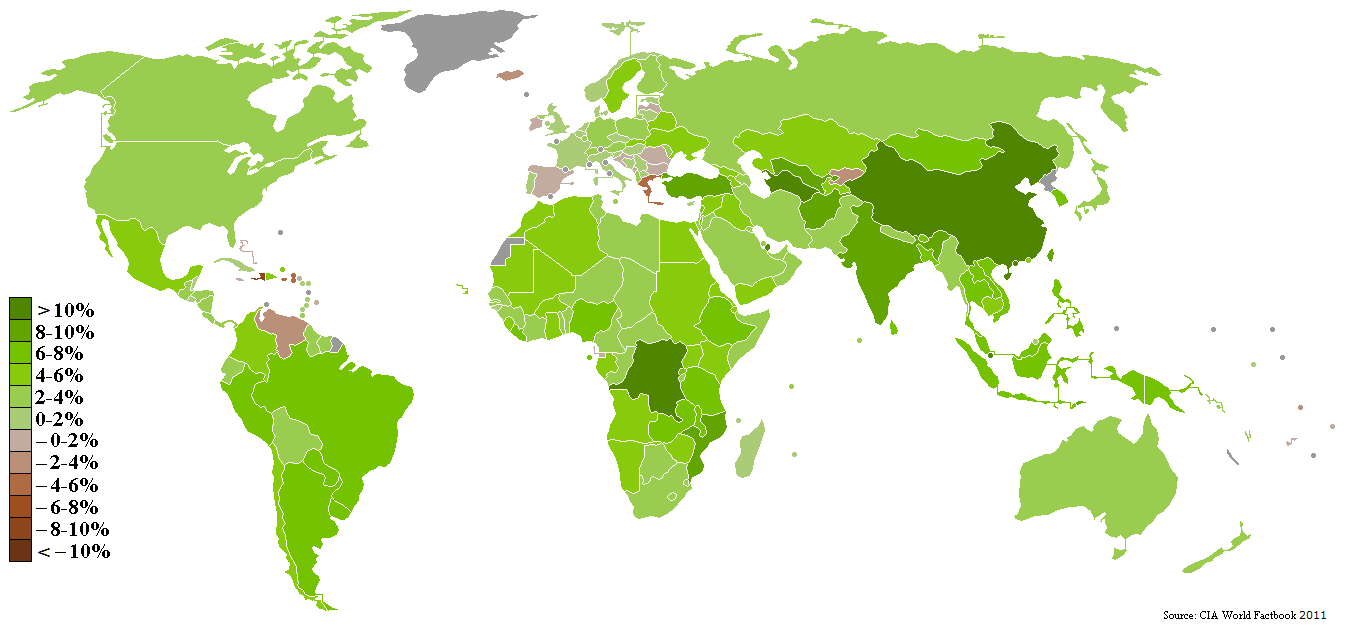
\includegraphics{img/gdp_rate_2007.png}
	\caption{Wzrost PKB w poszczególnych państwach w 2007 roku.\cite{CIA}}
	\label{gdp_rate_2007}
\end{figure}

Wzajemna nieufność instytucji finansowych poskutkował wstrzymaniem akcji kredytowej i zamrożeniem inwestycji. Światowe gospodarki pogrążyły się w recesji, czyli charakteryzował je ujemny przyrost PKB (kurczenie się gospodarki). Najmniej zostały dotknięte kraje arabskie, które w dużej mierze bazują na eksporcie surowców.

\subsubsection{Wpływ na rynek surowców naturalnych}

\begin{figure}[h] \centering %H if want to get it exaclty here
	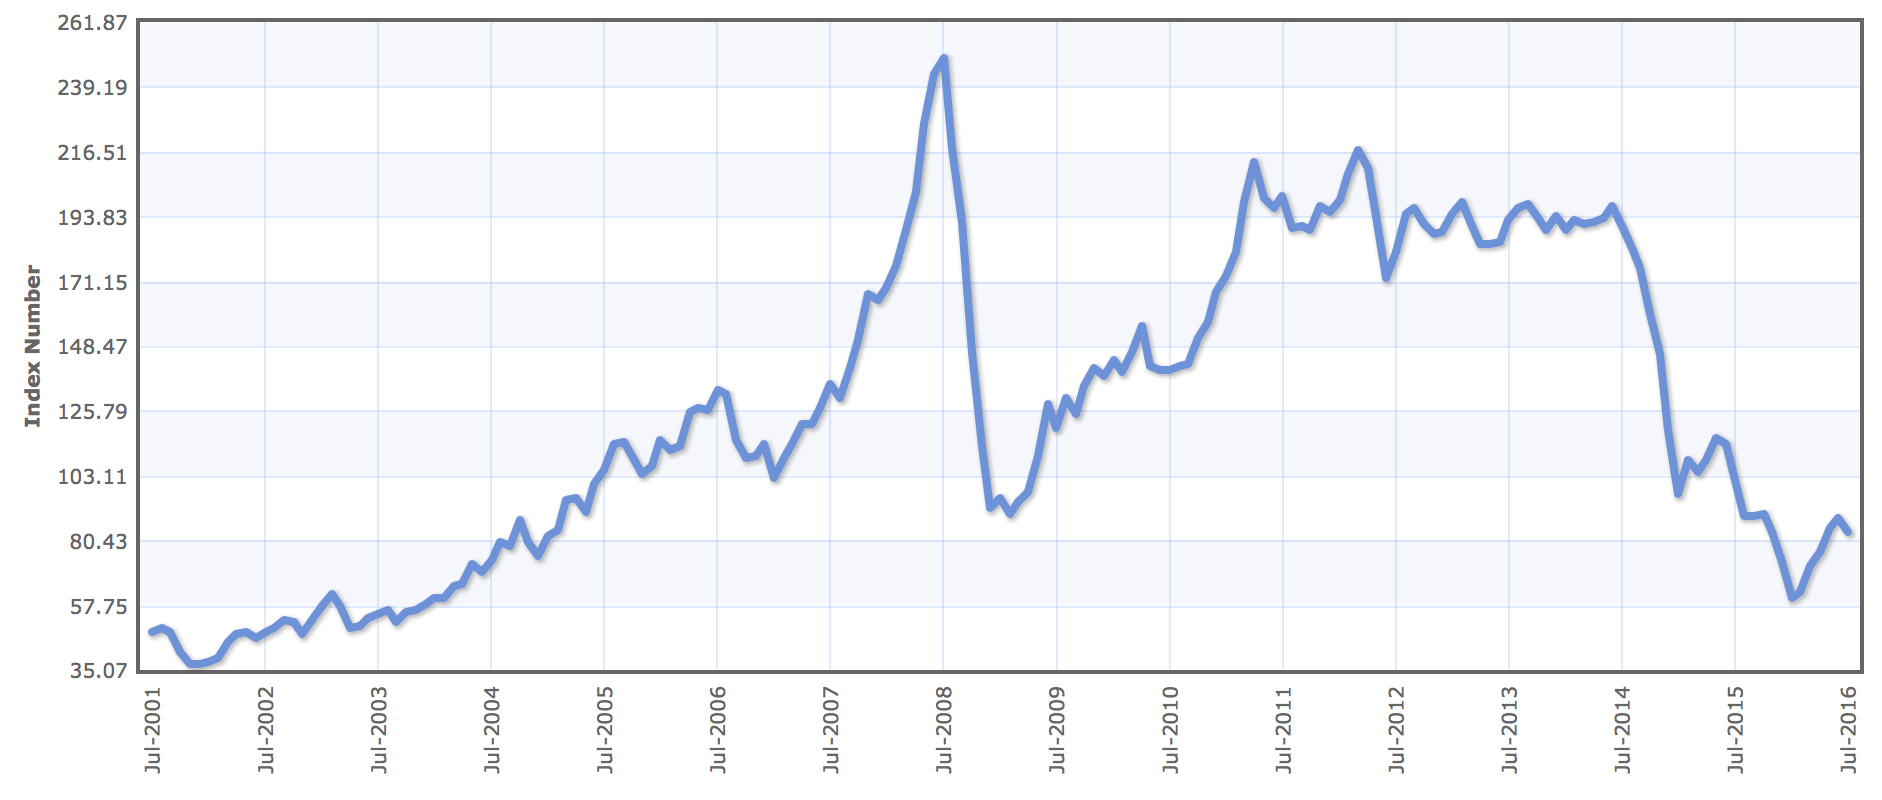
\includegraphics[scale=0.4]{img/fuel_index.png}
	\caption{Indeks cen paliw kopalnych latach 2001 - 2016.\cite{indexmundi}} %indexmundi.com
	\label{fuelPriceIndex}
\end{figure}

\begin{figure}[h] \centering %H if want to get it exaclty here
	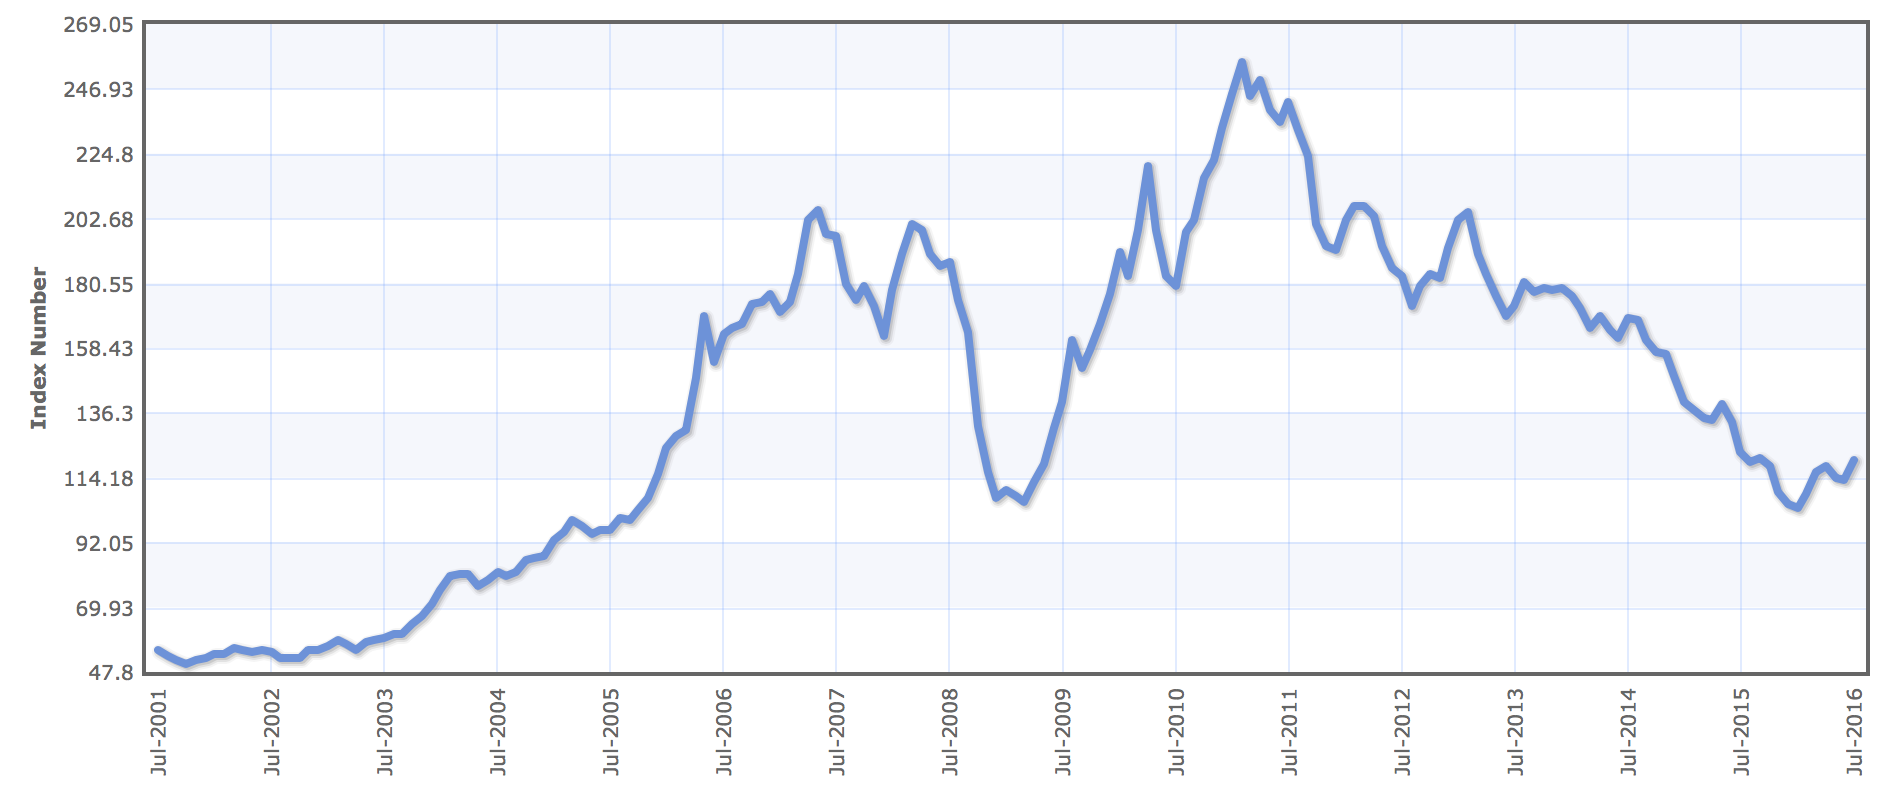
\includegraphics[scale=0.4]{img/metal_index.png}
	\caption{Indeks cen metali latach 2001 - 2016.\cite{indexmundi}} %indexmundi.com
	\label{metalPriceIndex}
\end{figure}

Wykresy przedstawione na rysunkachh 2.2 i 2.3 ukazują gwałtowny wzrost zainteresowania inwestycjami opartymi na surowcach naturalnych. Doprowadziło to do nienaturalnego, lecz chwilowego wzrostu cen - cena baryłki ropy wzrosła niemalże trzykrotnie na przestrzeni 18 miesięcy. Niestety ze względu na zamrożenie wielu inwestycji spowodowane brakiem kredytów po skoku cen nastąpił równie raptowny ich spadek. Przysporzyło to wielu problemów przedsiębiorstwom wydobywczym, m.in. doprowadziło do bankructwa wiele australijskich kopalni niklu.

\subsubsection{Wpływ na ceny żywności}

\begin{figure}[h] \centering %H if want to get it exaclty here
	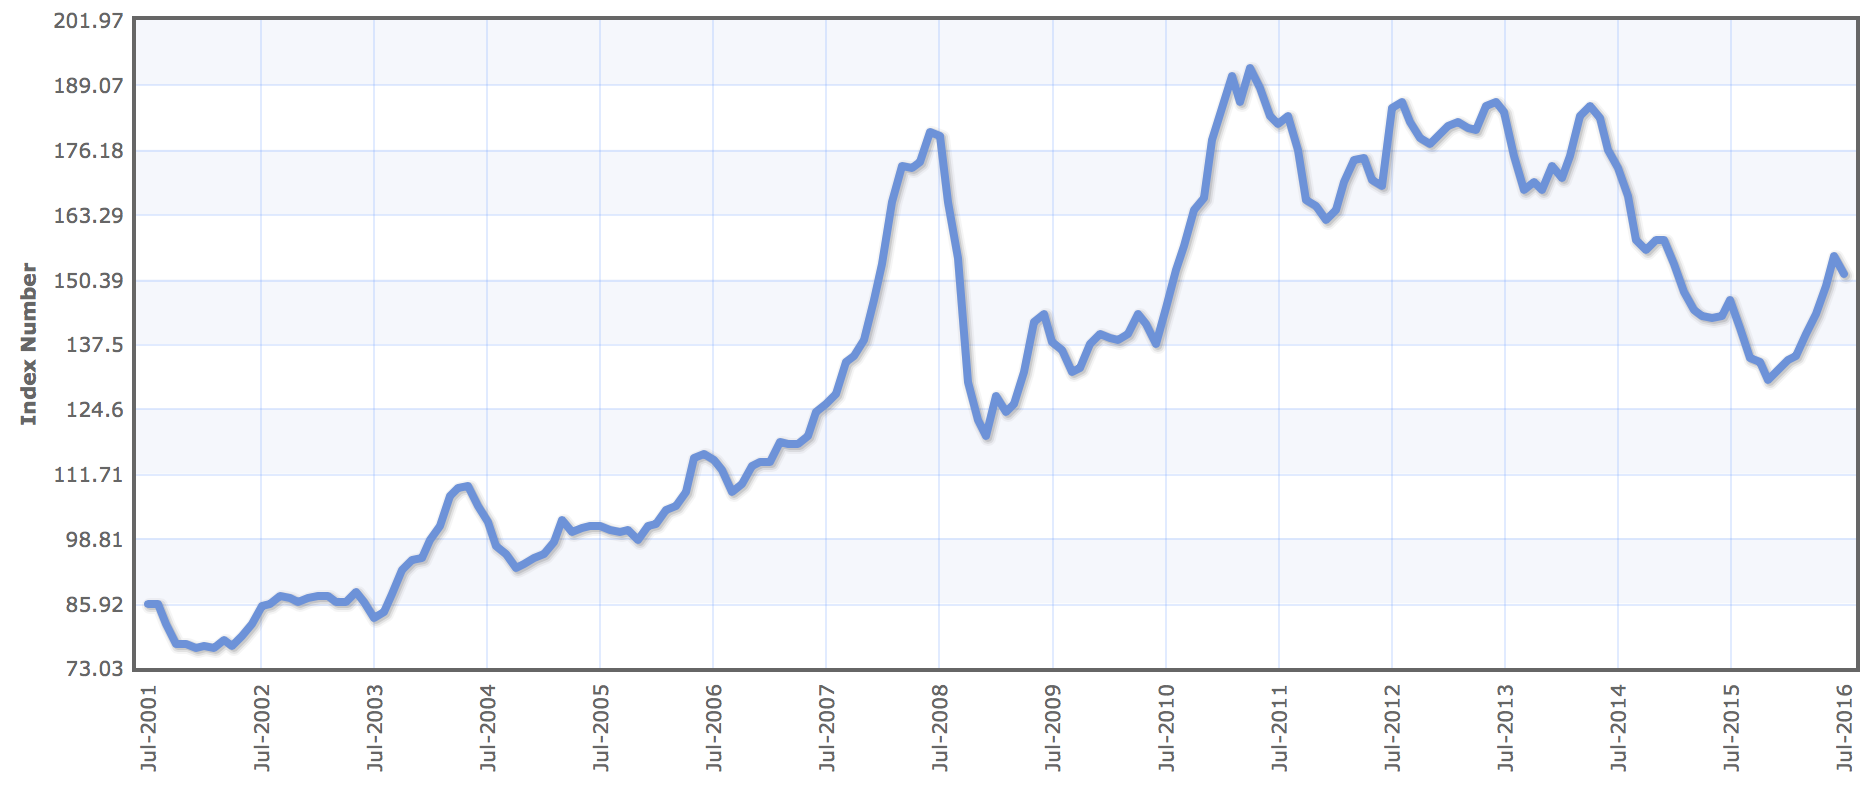
\includegraphics[scale=0.4]{img/food_index.png}
	\caption{Indeks cen żywności latach 2001 - 2016.\cite{indexmundi}} %indexmundi.com
	\label{foodPriceIndex}
\end{figure}

Jednym z tragicznych następstw kryzysu na rynkach finansowych był radykalny wzrost cen żywności. Najbardziej odczuły to kraje rozwijające się i tzw. Kraje Trzeciego Świata. Doprowadziło to do politycznej i ekonomicznej niestabilności w tych regionach.

\subsubsection{Bezrobocie}

Wzajemna nieufność instytucji finansowych poskutkował wstrzymaniem akcji kredytowej i zamrożenia inwestycji. Światowe gospodarki pogrążyły się w recesji, czyli charakteryzował je ujemny przyrost PKB (kurczenie się gospodarki). Najmniej zostały dotknięte kraje arabskie, które w dużej mierze bazują na eksporcie surowców.
za masowymi zwolnieniami w sektorze finansowym (w samej Wielkiej Brytanii pracę w tym sektorze straciło kilkadziesiąt tysięcy osób) ucierpiały również inne branże – przede wszystkim branża motoryzacyjna. Było to spowodowane załamaniem sprzedaży nowych samochodów finansowanej głównie za pomocą kredytów – a banki przestały ich udzielać.
Zadłużenie społeczeństwa i rosnące bezrobocie spowodowały spadek konsumpcji, co w sposób spiralny prowadziło do dalszego spadku produkcji i redukcji zatrudnienia.

\subsection{Walka z kryzysem}

Walka z kryzysem w dużej mierze sprowadzała się do dotowania instytucji sektora finansowego z pieniędzy podatników oraz stosowania praktyk protekcjonistycznych w stosunku do rodzimych firm – szczególnie dotyczyło to USA i Francji. W celu pobudzenia akcji kredytowej wprowadzono rekordowe obniżki stóp procentowych, co miało skłonić inwestorów do bardziej śmiałych i zdecydowanych działań.
Postanowiono wprowadzić nową normę: Basel III, która miała uchronić sektor finansowy przed popełnieniem tych samych błędów. Należy jednak pamiętać, że poprzednia odsłona tych regulacji – mylnie obwiniana za zaistniały kryzys – została ogłoszona w roku 2004, a w roku 2008 dopiero była wdrażana, czyli nie miała szansy realnie wpłynąć na kondycję ekonomiczną sektora bankowego i uchronić świata przed nadchodzącym gospodarczym tąpnięciem.
Rządy państw grupy G8 przekazały w sumie ponad 3 bln. \$ na cel ratowania własnych gospodarek. Postanowiono również zwiększyć rezerwy Międzynarodowego Funduszu Walutowego, a także planowano likwidację rajów podatkowych – pomysł ten nie doczekał się jednak realizacji.